\documentclass[../main.tex]{subfiles}


\begin{document}
%\begin{center}
%\begin{tabularx}{\textwidth}{|1|X|}
\begin{longtable}{| p{.20\textwidth} | p{.80\textwidth} |} 
\hline
    Kratak opis &  Recepcionar popunjava formular za registraciju novog korisnika na osnovu podataka koje dobija od korisnika koji je došao na recepciju.\\ 
\hline    
    Učesnici & 
         Recepcionar – Želi da efikasno izvši registraciju novog korisnika na sistem.
    \\
\hline
   Preduslovi & \begin{enumerate}
       \item Sistem je u funkciji.
       \item Recepcionar je ulogovan.
   \end{enumerate}\\
\hline  
    Postuslovi & \begin{enumerate}
        \item Korisniku je kreiran nalog i postao je klijent.
        \item Baza podataka je ažurirana.
    \end{enumerate}\\
\hline
    Osnovni tok & \begin{enumerate}
        \item Recepcionar u sistemu bira opciju za registraciju novog člana.
        \item Recepcionar u formular unosi osnovne podatke koje mu korisnik saopšti i pritiska dugme „Registruj korisnika“.
        \item Sistem vrši proveru podataka i šalje korisniku e-mail sa podacima.
        \item Sistem obaveštava recepcionara da je nalog aktiviran.
    \end{enumerate}\\
\hline
    Alternativni tokovi & \begin{itemize}
        \item[A3] Neuspešna provera podataka: Recepcionar ponovo uzima podatke od korisnika za neispravna polje. Slučaj se nastavlja na koraku 2.
    \end{itemize}\\
\hline
    Podtokovi & /\\
\hline
    Specijalni zahtevi & Korisnik mora da ima e-mail adresu.\\
\hline
    Dodatne informacije & \begin{itemize}
        \item Formular za registraciju od podataka zahteva: korisničko ime, ime, prezime, datum rođenja, e-mail, broj telefona, lozinku, polje za proveru lozinke.
        \item Podaci koje e-mailom sistem šalje korisniku: korisničko ime, lozinka i broj članske karte.
    \end{itemize} \\
\hline
%\end{tabularx}
%\end{center}    
\caption{Registracija uživo za neregistrovanog korisnika} % needs to go inside longtable environment
%\label{tab:myfirstlongtable}
\end{longtable}


%\begin{figure}[!ht]
%\begin{center}
%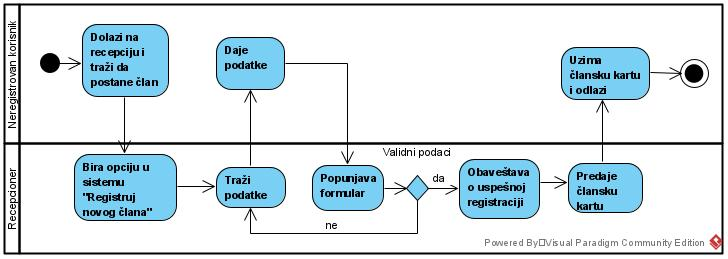
\includegraphics[scale=0.55]{sections/images/Dijagram_aktivnsti_registracije_uzivo.jpg}
%\end{center}
%\caption{Dijagram aktivnosti registracije uživo}
%\label{fig:kontekst}
%\end{figure}
\end{document}